\documentclass{article}
\usepackage[final,main]{neurips_2025}  % NEURIPS style (main track required to define footer)

\usepackage[utf8]{inputenc}
\usepackage[T1]{fontenc}
\usepackage[hidelinks]{hyperref}  % clickable links
\usepackage{booktabs}             % professional tables
\usepackage{graphicx}
\usepackage{amsmath,amssymb}
\usepackage{subcaption}
\usepackage{enumitem}
\usepackage{multirow}

% Import command files
\input{commands/math}
\input{commands/general}
%%%%% PROJECT-SPECIFIC MACROS %%%%%
% Define your project-specific terms here
% Import with: %%%%% PROJECT-SPECIFIC MACROS %%%%%
% Define your project-specific terms here
% Import with: %%%%% PROJECT-SPECIFIC MACROS %%%%%
% Define your project-specific terms here
% Import with: \input{commands/macros}
%
% INSTRUCTIONS:
% 1. Use \textsc{} for method/dataset/model names (small caps)
% 2. Add \xspace at the end for automatic spacing
% 3. Group related terms together
% 4. Use consistent naming conventions

\usepackage{xspace}

%%%%%%%%%%%%%%%%%%%%%%%%%%%%%%%%%%%%%%%%%%%%%%%%%%%%%%%%%%%%%%%%%
% MODEL NAMES
%%%%%%%%%%%%%%%%%%%%%%%%%%%%%%%%%%%%%%%%%%%%%%%%%%%%%%%%%%%%%%%%%

\newcommand{\qwenbig}{\textsc{Qwen2.5-7B-Instruct}\xspace}
\newcommand{\qwensmall}{\textsc{Qwen2.5-1.5B-Instruct}\xspace}

%%%%%%%%%%%%%%%%%%%%%%%%%%%%%%%%%%%%%%%%%%%%%%%%%%%%%%%%%%%%%%%%%
% DATASET NAMES
%%%%%%%%%%%%%%%%%%%%%%%%%%%%%%%%%%%%%%%%%%%%%%%%%%%%%%%%%%%%%%%%%

\newcommand{\goemotions}{\textsc{GoEmotions}\xspace}
\newcommand{\emobank}{\textsc{EmoBank}\xspace}
\newcommand{\dramacorpus}{\textsc{DramaReg}\xspace}

%%%%%%%%%%%%%%%%%%%%%%%%%%%%%%%%%%%%%%%%%%%%%%%%%%%%%%%%%%%%%%%%%
% NESTED MODEL NAMES
%%%%%%%%%%%%%%%%%%%%%%%%%%%%%%%%%%%%%%%%%%%%%%%%%%%%%%%%%%%%%%%%%

\newcommand{\Mzero}{\textsc{M0}\xspace}
\newcommand{\Mone}{\textsc{M1}\xspace}
\newcommand{\Mtwo}{\textsc{M2}\xspace}
\newcommand{\MtwoK}{\textsc{M2K}\xspace}
\newcommand{\Mthree}{\textsc{M3}\xspace}

%%%%%%%%%%%%%%%%%%%%%%%%%%%%%%%%%%%%%%%%%%%%%%%%%%%%%%%%%%%%%%%%%
% ABBREVIATIONS
%%%%%%%%%%%%%%%%%%%%%%%%%%%%%%%%%%%%%%%%%%%%%%%%%%%%%%%%%%%%%%%%%

\newcommand{\ie}{i.e.,\xspace}
\newcommand{\eg}{e.g.,\xspace}
\newcommand{\cf}{cf.\xspace}
\newcommand{\PR}{\textsc{pr}\xspace}

%%%%%%%%%%%%%%%%%%%%%%%%%%%%%%%%%%%%%%%%%%%%%%%%%%%%%%%%%%%%%%%%%
% DATASET NAMES
%%%%%%%%%%%%%%%%%%%%%%%%%%%%%%%%%%%%%%%%%%%%%%%%%%%%%%%%%%%%%%%%%

% Dataset names (use \textsc for consistency)
% Example: \newcommand{\datasetone}{\textsc{Dataset-One}\xspace}
% Example: \newcommand{\datasettwo}{\textsc{Dataset-Two}\xspace}

%%%%%%%%%%%%%%%%%%%%%%%%%%%%%%%%%%%%%%%%%%%%%%%%%%%%%%%%%%%%%%%%%
% MODEL NAMES
%%%%%%%%%%%%%%%%%%%%%%%%%%%%%%%%%%%%%%%%%%%%%%%%%%%%%%%%%%%%%%%%%

% LLM and model names
% Example: \newcommand{\gpt}{\textsc{GPT-4o-mini}\xspace}
% Example: \newcommand{\llama}{\textsc{Llama-3.1-70B-Instruct}\xspace}
% Example: \newcommand{\claude}{\textsc{Claude-3.5-Sonnet}\xspace}

%%%%%%%%%%%%%%%%%%%%%%%%%%%%%%%%%%%%%%%%%%%%%%%%%%%%%%%%%%%%%%%%%
% BASELINE NAMES
%%%%%%%%%%%%%%%%%%%%%%%%%%%%%%%%%%%%%%%%%%%%%%%%%%%%%%%%%%%%%%%%%

% Baseline method names
% Example: \newcommand{\baseline}{\textsc{BaselineMethod}\xspace}
% Example: \newcommand{\fewshot}{\textsc{Few-shot}\xspace}

%%%%%%%%%%%%%%%%%%%%%%%%%%%%%%%%%%%%%%%%%%%%%%%%%%%%%%%%%%%%%%%%%
% ABBREVIATIONS
%%%%%%%%%%%%%%%%%%%%%%%%%%%%%%%%%%%%%%%%%%%%%%%%%%%%%%%%%%%%%%%%%

% Common abbreviations used in your paper
% Example: \newcommand{\ie}{i.e.,\xspace}
% Example: \newcommand{\eg}{e.g.,\xspace}
% Example: \newcommand{\cf}{cf.\xspace}
% Example: \newcommand{\wrt}{w.r.t.\xspace}

%%%%%%%%%%%%%%%%%%%%%%%%%%%%%%%%%%%%%%%%%%%%%%%%%%%%%%%%%%%%%%%%%
% DOMAIN-SPECIFIC TERMS
%%%%%%%%%%%%%%%%%%%%%%%%%%%%%%%%%%%%%%%%%%%%%%%%%%%%%%%%%%%%%%%%%

% Terms specific to your research domain
% Keep consistent formatting throughout the paper

%%%%%%%%%%%%%%%%%%%%%%%%%%%%%%%%%%%%%%%%%%%%%%%%%%%%%%%%%%%%%%%%%
% USAGE EXAMPLES
%%%%%%%%%%%%%%%%%%%%%%%%%%%%%%%%%%%%%%%%%%%%%%%%%%%%%%%%%%%%%%%%%
%
% GOOD:
%   \newcommand{\hypogenic}{\textsc{HypoGeniC}\xspace}
%   Usage: "We propose \hypogenic to generate hypotheses."
%   Result: "We propose HypoGeniC to generate hypotheses."
%
% GOOD:
%   \newcommand{\ours}{{\bf HypoGeniC}\xspace}
%   Usage: "Our method, \ours, outperforms baselines."
%   Result: "Our method, HypoGeniC, outperforms baselines."
%
% BAD (no \xspace):
%   \newcommand{\hypogenic}{\textsc{HypoGeniC}}
%   Usage: "\hypogenic outperforms..."
%   Result: "HypoGeniCoutperforms..." (missing space!)
%
%%%%%%%%%%%%%%%%%%%%%%%%%%%%%%%%%%%%%%%%%%%%%%%%%%%%%%%%%%%%%%%%%

%
% INSTRUCTIONS:
% 1. Use \textsc{} for method/dataset/model names (small caps)
% 2. Add \xspace at the end for automatic spacing
% 3. Group related terms together
% 4. Use consistent naming conventions

\usepackage{xspace}

%%%%%%%%%%%%%%%%%%%%%%%%%%%%%%%%%%%%%%%%%%%%%%%%%%%%%%%%%%%%%%%%%
% MODEL NAMES
%%%%%%%%%%%%%%%%%%%%%%%%%%%%%%%%%%%%%%%%%%%%%%%%%%%%%%%%%%%%%%%%%

\newcommand{\qwenbig}{\textsc{Qwen2.5-7B-Instruct}\xspace}
\newcommand{\qwensmall}{\textsc{Qwen2.5-1.5B-Instruct}\xspace}

%%%%%%%%%%%%%%%%%%%%%%%%%%%%%%%%%%%%%%%%%%%%%%%%%%%%%%%%%%%%%%%%%
% DATASET NAMES
%%%%%%%%%%%%%%%%%%%%%%%%%%%%%%%%%%%%%%%%%%%%%%%%%%%%%%%%%%%%%%%%%

\newcommand{\goemotions}{\textsc{GoEmotions}\xspace}
\newcommand{\emobank}{\textsc{EmoBank}\xspace}
\newcommand{\dramacorpus}{\textsc{DramaReg}\xspace}

%%%%%%%%%%%%%%%%%%%%%%%%%%%%%%%%%%%%%%%%%%%%%%%%%%%%%%%%%%%%%%%%%
% NESTED MODEL NAMES
%%%%%%%%%%%%%%%%%%%%%%%%%%%%%%%%%%%%%%%%%%%%%%%%%%%%%%%%%%%%%%%%%

\newcommand{\Mzero}{\textsc{M0}\xspace}
\newcommand{\Mone}{\textsc{M1}\xspace}
\newcommand{\Mtwo}{\textsc{M2}\xspace}
\newcommand{\MtwoK}{\textsc{M2K}\xspace}
\newcommand{\Mthree}{\textsc{M3}\xspace}

%%%%%%%%%%%%%%%%%%%%%%%%%%%%%%%%%%%%%%%%%%%%%%%%%%%%%%%%%%%%%%%%%
% ABBREVIATIONS
%%%%%%%%%%%%%%%%%%%%%%%%%%%%%%%%%%%%%%%%%%%%%%%%%%%%%%%%%%%%%%%%%

\newcommand{\ie}{i.e.,\xspace}
\newcommand{\eg}{e.g.,\xspace}
\newcommand{\cf}{cf.\xspace}
\newcommand{\PR}{\textsc{pr}\xspace}

%%%%%%%%%%%%%%%%%%%%%%%%%%%%%%%%%%%%%%%%%%%%%%%%%%%%%%%%%%%%%%%%%
% DATASET NAMES
%%%%%%%%%%%%%%%%%%%%%%%%%%%%%%%%%%%%%%%%%%%%%%%%%%%%%%%%%%%%%%%%%

% Dataset names (use \textsc for consistency)
% Example: \newcommand{\datasetone}{\textsc{Dataset-One}\xspace}
% Example: \newcommand{\datasettwo}{\textsc{Dataset-Two}\xspace}

%%%%%%%%%%%%%%%%%%%%%%%%%%%%%%%%%%%%%%%%%%%%%%%%%%%%%%%%%%%%%%%%%
% MODEL NAMES
%%%%%%%%%%%%%%%%%%%%%%%%%%%%%%%%%%%%%%%%%%%%%%%%%%%%%%%%%%%%%%%%%

% LLM and model names
% Example: \newcommand{\gpt}{\textsc{GPT-4o-mini}\xspace}
% Example: \newcommand{\llama}{\textsc{Llama-3.1-70B-Instruct}\xspace}
% Example: \newcommand{\claude}{\textsc{Claude-3.5-Sonnet}\xspace}

%%%%%%%%%%%%%%%%%%%%%%%%%%%%%%%%%%%%%%%%%%%%%%%%%%%%%%%%%%%%%%%%%
% BASELINE NAMES
%%%%%%%%%%%%%%%%%%%%%%%%%%%%%%%%%%%%%%%%%%%%%%%%%%%%%%%%%%%%%%%%%

% Baseline method names
% Example: \newcommand{\baseline}{\textsc{BaselineMethod}\xspace}
% Example: \newcommand{\fewshot}{\textsc{Few-shot}\xspace}

%%%%%%%%%%%%%%%%%%%%%%%%%%%%%%%%%%%%%%%%%%%%%%%%%%%%%%%%%%%%%%%%%
% ABBREVIATIONS
%%%%%%%%%%%%%%%%%%%%%%%%%%%%%%%%%%%%%%%%%%%%%%%%%%%%%%%%%%%%%%%%%

% Common abbreviations used in your paper
% Example: \newcommand{\ie}{i.e.,\xspace}
% Example: \newcommand{\eg}{e.g.,\xspace}
% Example: \newcommand{\cf}{cf.\xspace}
% Example: \newcommand{\wrt}{w.r.t.\xspace}

%%%%%%%%%%%%%%%%%%%%%%%%%%%%%%%%%%%%%%%%%%%%%%%%%%%%%%%%%%%%%%%%%
% DOMAIN-SPECIFIC TERMS
%%%%%%%%%%%%%%%%%%%%%%%%%%%%%%%%%%%%%%%%%%%%%%%%%%%%%%%%%%%%%%%%%

% Terms specific to your research domain
% Keep consistent formatting throughout the paper

%%%%%%%%%%%%%%%%%%%%%%%%%%%%%%%%%%%%%%%%%%%%%%%%%%%%%%%%%%%%%%%%%
% USAGE EXAMPLES
%%%%%%%%%%%%%%%%%%%%%%%%%%%%%%%%%%%%%%%%%%%%%%%%%%%%%%%%%%%%%%%%%
%
% GOOD:
%   \newcommand{\hypogenic}{\textsc{HypoGeniC}\xspace}
%   Usage: "We propose \hypogenic to generate hypotheses."
%   Result: "We propose HypoGeniC to generate hypotheses."
%
% GOOD:
%   \newcommand{\ours}{{\bf HypoGeniC}\xspace}
%   Usage: "Our method, \ours, outperforms baselines."
%   Result: "Our method, HypoGeniC, outperforms baselines."
%
% BAD (no \xspace):
%   \newcommand{\hypogenic}{\textsc{HypoGeniC}}
%   Usage: "\hypogenic outperforms..."
%   Result: "HypoGeniCoutperforms..." (missing space!)
%
%%%%%%%%%%%%%%%%%%%%%%%%%%%%%%%%%%%%%%%%%%%%%%%%%%%%%%%%%%%%%%%%%

%
% INSTRUCTIONS:
% 1. Use \textsc{} for method/dataset/model names (small caps)
% 2. Add \xspace at the end for automatic spacing
% 3. Group related terms together
% 4. Use consistent naming conventions

\usepackage{xspace}

%%%%%%%%%%%%%%%%%%%%%%%%%%%%%%%%%%%%%%%%%%%%%%%%%%%%%%%%%%%%%%%%%
% MODEL NAMES
%%%%%%%%%%%%%%%%%%%%%%%%%%%%%%%%%%%%%%%%%%%%%%%%%%%%%%%%%%%%%%%%%

\newcommand{\qwenbig}{\textsc{Qwen2.5-7B-Instruct}\xspace}
\newcommand{\qwensmall}{\textsc{Qwen2.5-1.5B-Instruct}\xspace}

%%%%%%%%%%%%%%%%%%%%%%%%%%%%%%%%%%%%%%%%%%%%%%%%%%%%%%%%%%%%%%%%%
% DATASET NAMES
%%%%%%%%%%%%%%%%%%%%%%%%%%%%%%%%%%%%%%%%%%%%%%%%%%%%%%%%%%%%%%%%%

\newcommand{\goemotions}{\textsc{GoEmotions}\xspace}
\newcommand{\emobank}{\textsc{EmoBank}\xspace}
\newcommand{\dramacorpus}{\textsc{DramaReg}\xspace}

%%%%%%%%%%%%%%%%%%%%%%%%%%%%%%%%%%%%%%%%%%%%%%%%%%%%%%%%%%%%%%%%%
% NESTED MODEL NAMES
%%%%%%%%%%%%%%%%%%%%%%%%%%%%%%%%%%%%%%%%%%%%%%%%%%%%%%%%%%%%%%%%%

\newcommand{\Mzero}{\textsc{M0}\xspace}
\newcommand{\Mone}{\textsc{M1}\xspace}
\newcommand{\Mtwo}{\textsc{M2}\xspace}
\newcommand{\MtwoK}{\textsc{M2K}\xspace}
\newcommand{\Mthree}{\textsc{M3}\xspace}

%%%%%%%%%%%%%%%%%%%%%%%%%%%%%%%%%%%%%%%%%%%%%%%%%%%%%%%%%%%%%%%%%
% ABBREVIATIONS
%%%%%%%%%%%%%%%%%%%%%%%%%%%%%%%%%%%%%%%%%%%%%%%%%%%%%%%%%%%%%%%%%

\newcommand{\ie}{i.e.,\xspace}
\newcommand{\eg}{e.g.,\xspace}
\newcommand{\cf}{cf.\xspace}
\newcommand{\PR}{\textsc{pr}\xspace}

%%%%%%%%%%%%%%%%%%%%%%%%%%%%%%%%%%%%%%%%%%%%%%%%%%%%%%%%%%%%%%%%%
% DATASET NAMES
%%%%%%%%%%%%%%%%%%%%%%%%%%%%%%%%%%%%%%%%%%%%%%%%%%%%%%%%%%%%%%%%%

% Dataset names (use \textsc for consistency)
% Example: \newcommand{\datasetone}{\textsc{Dataset-One}\xspace}
% Example: \newcommand{\datasettwo}{\textsc{Dataset-Two}\xspace}

%%%%%%%%%%%%%%%%%%%%%%%%%%%%%%%%%%%%%%%%%%%%%%%%%%%%%%%%%%%%%%%%%
% MODEL NAMES
%%%%%%%%%%%%%%%%%%%%%%%%%%%%%%%%%%%%%%%%%%%%%%%%%%%%%%%%%%%%%%%%%

% LLM and model names
% Example: \newcommand{\gpt}{\textsc{GPT-4o-mini}\xspace}
% Example: \newcommand{\llama}{\textsc{Llama-3.1-70B-Instruct}\xspace}
% Example: \newcommand{\claude}{\textsc{Claude-3.5-Sonnet}\xspace}

%%%%%%%%%%%%%%%%%%%%%%%%%%%%%%%%%%%%%%%%%%%%%%%%%%%%%%%%%%%%%%%%%
% BASELINE NAMES
%%%%%%%%%%%%%%%%%%%%%%%%%%%%%%%%%%%%%%%%%%%%%%%%%%%%%%%%%%%%%%%%%

% Baseline method names
% Example: \newcommand{\baseline}{\textsc{BaselineMethod}\xspace}
% Example: \newcommand{\fewshot}{\textsc{Few-shot}\xspace}

%%%%%%%%%%%%%%%%%%%%%%%%%%%%%%%%%%%%%%%%%%%%%%%%%%%%%%%%%%%%%%%%%
% ABBREVIATIONS
%%%%%%%%%%%%%%%%%%%%%%%%%%%%%%%%%%%%%%%%%%%%%%%%%%%%%%%%%%%%%%%%%

% Common abbreviations used in your paper
% Example: \newcommand{\ie}{i.e.,\xspace}
% Example: \newcommand{\eg}{e.g.,\xspace}
% Example: \newcommand{\cf}{cf.\xspace}
% Example: \newcommand{\wrt}{w.r.t.\xspace}

%%%%%%%%%%%%%%%%%%%%%%%%%%%%%%%%%%%%%%%%%%%%%%%%%%%%%%%%%%%%%%%%%
% DOMAIN-SPECIFIC TERMS
%%%%%%%%%%%%%%%%%%%%%%%%%%%%%%%%%%%%%%%%%%%%%%%%%%%%%%%%%%%%%%%%%

% Terms specific to your research domain
% Keep consistent formatting throughout the paper

%%%%%%%%%%%%%%%%%%%%%%%%%%%%%%%%%%%%%%%%%%%%%%%%%%%%%%%%%%%%%%%%%
% USAGE EXAMPLES
%%%%%%%%%%%%%%%%%%%%%%%%%%%%%%%%%%%%%%%%%%%%%%%%%%%%%%%%%%%%%%%%%
%
% GOOD:
%   \newcommand{\hypogenic}{\textsc{HypoGeniC}\xspace}
%   Usage: "We propose \hypogenic to generate hypotheses."
%   Result: "We propose HypoGeniC to generate hypotheses."
%
% GOOD:
%   \newcommand{\ours}{{\bf HypoGeniC}\xspace}
%   Usage: "Our method, \ours, outperforms baselines."
%   Result: "Our method, HypoGeniC, outperforms baselines."
%
% BAD (no \xspace):
%   \newcommand{\hypogenic}{\textsc{HypoGeniC}}
%   Usage: "\hypogenic outperforms..."
%   Result: "HypoGeniCoutperforms..." (missing space!)
%
%%%%%%%%%%%%%%%%%%%%%%%%%%%%%%%%%%%%%%%%%%%%%%%%%%%%%%%%%%%%%%%%%


\bibliographystyle{plainnat}

\title{Different Kinds of Drama: Drama Is a Multi-Dimensional Construct\\ but Reader Disagreement Is a Threshold on a Shared Axis}

\author{Ari Holtzman and NeuriCo}

\begin{document}
\maketitle

\begin{abstract}
When a language model judges a piece of text as gripping, overwrought, or merely flat, it makes an affect-laden subjective call, and different readers will not agree on it. The distinction between drama and \emph{melodrama} sharpens the question: is melodrama simply more drama, or something categorically different, and does reader disagreement live on the same axis? No prior work studies how models represent drama; the broader debate over whether subjective constructs are single directions or multi-dimensional subspaces remains unsettled, and model-internal affect geometry has never been joined to per-reader behavioral variation. We probe the representation geometry of Qwen2.5-7B and 1.5B using a controlled, blind-validated drama corpus and 70 identified GoEmotions raters, with difference-in-means directions, participation-ratio estimates of subspace dimension, and nested held-out logistic models gauged against a shuffled-reader null. We find a clean dissociation. The construct is multi-dimensional: drama decodes at AUROC 1.00, yet the step to melodrama rotates to roughly 83 degrees off the drama axis (subspace participation ratio about 5.6), so melodrama lives on a distinct excess direction. Reader variation, by contrast, is a sliding threshold: adding a per-reader threshold lifts held-out AUROC from 0.51 to 0.62 and 0.66 to 0.70, while letting each reader pick their own direction adds exactly the shuffled-reader null, and six prompted personas leave the drama axis fixed at cosine at least 0.97. Different kinds of drama live in shared content; different people mostly move a threshold.

\end{abstract}

\section{Introduction}\label{sec:intro}

Language models increasingly make affect-laden subjective judgments: they moderate emotionally charged posts, co-author stories, hold companionship-style conversations, and critique creative work. All of these tasks hinge on a model's internal sense of how \emph{dramatic} a piece of text is---and on whether that sense matches the reader being served. But ``dramatic'' is not one thing. A war memoir and a soap-opera confession can be equally intense while differing in kind: one earns its intensity, the other piles it on. If a model collapses drama onto a single intensity axis, it conflates earned drama with melodramatic excess, and it mis-models readers who disagree not about \emph{how much} drama a text has but about \emph{what kind} they are willing to credit. Knowing whether a model's affect representation has the right shape---and whether reader disagreement lives in that shape---is a prerequisite for steering, auditing, or personalizing any of these systems.

\para{The problem.} Two questions are tangled together in practice. First, is the \emph{construct} of drama one-dimensional or many? Whether melodrama is ``just more drama'' or a qualitatively distinct register determines whether a single learned ``drama'' direction can faithfully control affective tone. Second, where does \emph{reader} disagreement come from? When two annotators split on whether a passage is dramatic, are they reading along a different internal direction (a difference in kind), or sharing the same axis and merely placing their cutoff in a different spot (a difference in degree)? These have opposite engineering consequences---personalization by re-aiming a direction versus personalization by shifting a threshold---yet they are routinely conflated.

\para{The gap.} No prior work studies ``drama'' as a model-internal construct, nor the dramatic-versus-melodramatic contrast. The closely related single-direction-versus-subspace question is unsettled even for the best-studied concept, refusal: \citet{arditi2024refusal} report a single mediating direction, while \citet{wollschlager2025geometry} argue for a multi-dimensional concept cone. Separately, work on emotion shows that affect occupies a low-dimensional manifold in representation space \citep{reichman2025emotions}, and work on annotation shows that reader effects are real and large \citep{orlikowski2025beyond,zhou2025subjectivity}. But model-internal affect geometry has never been joined to per-reader behavioral variation: we do not know whether the dimensions a model uses to represent affect are the same dimensions along which readers actually disagree.

\para{Our approach.} We separate the geometry of the drama \emph{construct} from the geometry of \emph{reader} variation, and we state two precise hypotheses. \textbf{H1 (single-axis limit):} the dramatic-versus-melodramatic distinction and reader variation in it are thresholds and regions on a low-dimensional shared drama-feature space---in the limit, one drama axis plus a per-reader threshold. \textbf{H2 (reader directions):} reader variation is a reader-specific \emph{direction} within a multi-dimensional drama subspace, so different readers read along different axes. We test these with difference-in-means directions \citep{marks2023geometry} over hidden states of \qwenbig (replicated in \qwensmall), using a controlled, blind-validated drama corpus (\dramacorpus) for construct geometry and a 70-reader \goemotions setup for behavioral disagreement. As a teaser, \figref{fig:excess} shows the key construct result: dramatic and melodramatic texts sit at the \emph{same} value on the drama axis but split along an orthogonal ``excess'' axis.

\para{Findings.} Our result splits cleanly across the two questions. The \emph{construct} is genuinely multi-dimensional, refuting the single-axis limit: drama itself decodes perfectly (AUROC $1.00$), yet melodrama is not just more drama---the dramatic$\rightarrow$melodramatic step rotates to $\sim\!83^\circ$ (nearly orthogonal) to the drama axis in deep layers, and an 8-subconcept subspace has participation ratio rising to $\sim\!5.6$ (versus $\sim\!8.0$ for random directions and $1$ for a single axis). \emph{Reader} variation, in sharp contrast, is overwhelmingly a threshold on a shared low-dimensional axis (H1). Adding a per-reader threshold to a shared single axis lifts held-out AUROC from $0.51$ to $0.62$ on the transferred corpus subspace and from $0.66$ to $0.70$ in domain---while letting each reader choose their \emph{own} direction adds exactly the shuffled-reader null ($\Delta$AUROC $+0.0076$ real versus $+0.0076$ null, $z\!\approx\!1.0$, n.s.). Six prompted reader personas leave the drama axis essentially fixed (pairwise cosine $\geq 0.97$, mean $0.99$). In one sentence: {\bf drama is multi-dimensional and shared across readers, but people mostly differ in \emph{where} they put the threshold, not in \emph{which direction} they read.}

\para{Contributions.} We make the following contributions:
\begin{itemize}[leftmargin=*,itemsep=0pt,topsep=0pt]
\item We build \dramacorpus, a validated controlled drama corpus (24 scenarios $\times$ 4 registers plus 8 drama subconcepts, blind re-labeled at $100\%$ agreement), and a per-reader \goemotions setup (70 raters, 56{,}995 texts, $36\%$ contested), jointly enabling construct and reader geometry to be measured on the same model internals.
\item We show the drama construct is multi-dimensional: drama decodes at AUROC $1.00$, but melodrama lives on an orthogonal excess axis ($\sim\!83^\circ$, subspace PR $\sim\!5.6$), so melodrama is not just more drama (\figref{fig:excess}).
\item We show reader variation is a \emph{threshold, not a direction}, via nested held-out logistic models against a shuffled-reader permutation null: the decisive lift is adding a per-reader threshold ($+0.04$ to $+0.11$), while reader-specific directions add nothing beyond the null, replicated across scales ($1.5$B/$7$B) and layers.
\item We corroborate with a persona probe: re-deriving the drama axis under six prompted reader personas leaves its direction unchanged (pairwise cosine $\geq 0.97$), shifting projection and threshold rather than axis.
\end{itemize}

We review related work in \secref{sec:related}, detail our corpus, models, and nested-model protocol in \secref{sec:method}, present the construct and reader-variation experiments in \secref{sec:results}, and discuss implications for steering and personalization in \secref{sec:discussion}.

\section{Related Work}\label{sec:related}

\para{Linear representations: single direction vs.\ subspace.}
A large body of work shows that high-level concepts are encoded as linear directions in LLM activation space. \citet{park2023linear} formalize the linear representation hypothesis, \citet{tigges2023linear} localize sentiment to a single direction, and \citet{arditi2024refusal} show that refusal is mediated by one direction. \citet{marks2023geometry} establish that difference-in-means directions are both robust and causal, the estimator we adopt throughout. A competing line argues that many concepts occupy a multi-dimensional \emph{subspace} rather than a single axis: \citet{wollschlager2025geometry} describe concept cones, \citet{zhao2024gcs} fit Gaussian concept subspaces, \citet{shafran2026regions} characterize concepts as regions amenable to multi-feature analysis, and \citet{shah2025harmfulness} probe subconcepts to recover a low-rank harmfulness subspace, a template we adapt to build the drama subspace. \citet{subramani2022steering} steer generation along extracted directions. Unlike this work, which adjudicates single-axis versus subspace on factual or behavioral concepts, we test the geometry of a fresh, evaluative, reader-dependent construct, and we do so \emph{separately} for the construct itself and for the variation across readers.

\para{Structured and relational probes.}
Beyond single directions, probes can recover structured and relational geometry. \citet{hewitt2019structural} extract syntax trees, \citet{nanda2023emergent} find emergent world models, and \citet{marks2024sfc} attribute behavior through sparse feature circuits. \citet{dawes2026hprobes} probe conceptual hierarchy, \citet{kozlowski2026semantic} show that evaluative axes live on a shared low-dimensional subspace with cross-axis spillover, and \citet{lee2026tpr} factorize representations along a reader $\times$ content structure. These results directly motivate our central test: whether reader variation factorizes as a reader $\times$ drama interaction (H2). Building on this framing, we operationalize and test that factorization explicitly, and find it absent.

\para{Affect geometry in LLMs.}
Closest in subject matter, recent work maps the geometry of affect inside LLMs. \citet{reichman2025emotions} find a low-dimensional, steerable emotional manifold and introduce a synthetic-to-real transfer protocol that we reuse to validate our controlled corpus against naturalistic data. \citet{wang2025emotion} localize emotion circuits, and \citet{zhao2025hierarchical} describe a hierarchical, persona-biased emotional representation. This evidence supports the low-dimensional premise underlying H1. We extend it with a reader-conditioning test that asks not just how affect is represented, but how the representation of what is \emph{dramatic} varies across the people perceiving it.

\para{Perspective and reader axes.}
A reader's viewpoint can itself be a low-dimensional direction. \citet{kim2025political} recover a political-perspective axis, and \citet{qin2026granularity} find a role-granularity axis governing how models adopt perspectives. Unlike these studies, which establish that a perspective axis exists, we ask whether such a reader axis \emph{hosts} a drama subspace, that is, whether different readers read drama along different directions or merely set different thresholds on a shared one.

\para{Subjectivity and per-reader modeling.}
Annotation-disagreement research treats reader variation as signal rather than noise. \citet{song2025survey} survey learning with disagreement; \citet{orlikowski2025beyond} show that reader effects are largely idiosyncratic rather than demographic; and \citet{kanclerz2022personalized,kanclerz2023pals,bielaniewicz2023chuckles} build personalized models of subjective phenomena including humor. \citet{mehrotra2026multi}, \citet{zhou2025subjectivity}, \citet{mieleszczenko2023capturing}, and \citet{alexeeva2023annotating} further model per-annotator labels and contested items. This work establishes that reader identity carries large, learnable variance that is not reducible to low-dimensional demographics, which we confirm in the strong per-reader threshold effect. Adding to it, we show in representation space that this variance is also not a reader-specific drama \emph{direction}: readers differ in where they place a threshold, not in which way they read.

\para{Narrative drama and reader response.}
Finally, computational narrative work grounds our construct. \citet{tian2024narratives} and \citet{christ2024emotional} model arousal and suspense trajectories, \citet{subbiah2025spinning} study narrative ambiguity, and \citet{dai2026cedar} document cross-cultural divergence in affective response. We operationalize drama as perceived emotional intensity in this tradition, drawing labels from \goemotions \citep{demszky2020goemotions} and inspecting \emobank \citep{buechel2017emobank} as auxiliary aggregate evidence. Unlike this work, which studies drama and reader response behaviorally, we connect it to the internal geometry of an LLM.

\section{Methodology}\label{sec:method}

We separate two questions that are easy to conflate: how the model represents the \emph{drama construct} itself, and how it represents \emph{reader variation} in drama. Our experiments are designed so that one set isolates the geometry of the construct (E1, E2, E4) and a second set isolates the geometry of disagreement (E3). We describe the hypotheses, the model and extraction pipeline, the two data sources, the five experiments, and the metrics and controls.

\para{Hypotheses.} We test two accounts of how \qwenbig encodes what different people find dramatic. Under \textbf{H1}, drama is a low-dimensional shared feature space, and readers differ by \emph{thresholds or regions} on that space rather than by what they read; in the single-axis limit this reduces to one drama axis plus a per-reader threshold (intercept). Under \textbf{H2}, readers differ by a \emph{reader-specific direction} inside a multi-dimensional drama subspace, so that two people can disagree because they project the same activations onto different drama features. These hypotheses concern two distinct geometries, and we keep them apart on purpose: the construct can be multi-dimensional while reader variation is still a one-dimensional threshold effect, which is in fact what we find. We pre-registered the decision rule. \textbf{H2} is supported \emph{iff} (i) the melodrama residual is decodable above a control \emph{and} (ii) the held-out AUROC gain from giving each reader their own direction, $\Delta\mathrm{AUROC}(\Mthree-\Mtwo)$, has a bootstrap 95\% CI that excludes zero. \textbf{H1} is supported \emph{iff} \Mone${\approx}$\Mtwo${\approx}$\Mthree and the melodrama residual matches its control. The construct-geometry sub-hypotheses (single axis vs.\ multi-dimensional space) are evaluated separately from the reader-variation sub-hypotheses (threshold vs.\ direction).

\para{Models and activation extraction.} Our primary model is \qwenbig (28 layers, hidden size 3584); we replicate the full pipeline on \qwensmall (28 layers, hidden size 1536) as a scale ablation. We run both from HuggingFace in \texttt{bfloat16} on a single RTX A6000; \texttt{fp16} produced NaNs in the deep layers, which we document and avoid. For each text we take hidden states and mean-pool over the text tokens, extracting at layers spanning relative depths $\{0.25, 0.5, 0.57, 0.75, 1.0\}$. We use raw text for all base-geometry experiments (E1--E3) and the chat template with a system persona for the persona probe (E4). All concept directions are difference-in-means vectors, which are robust and causally meaningful~\citep{marks2023geometry}: for a binary contrast with positive and negative example sets, the direction is
\[
\mathbf{v} \;=\; \boldsymbol{\mu}_{+} - \boldsymbol{\mu}_{-},
\qquad
\boldsymbol{\mu}_{\pm} = \tfrac{1}{|S_{\pm}|}\sum_{x \in S_{\pm}} h_\ell(x),
\]
where $h_\ell(x)$ is the mean-pooled activation at layer $\ell$. We fix all seeds to 42. APIs are used only for stimulus generation and validation; every model-internal computation runs locally on the GPU.

\para{Controlled drama corpus (\dramacorpus).} To probe construct geometry under tight control, we build \dramacorpus. It contains 24 base scenarios crossed with 4 registers $\{$neutral, understated, dramatic, melodramatic$\}$ for 96 register-matched texts, plus 8 drama subconcepts (suspense, pathos/grief, spectacle, stakes, sincerity, excess/sentimentality, shock, restraint), each with ${\sim}24$ contrast texts, for 194 additional texts. The corpus is produced by a 28-agent generation workflow and then adversarially blind re-labeled by independent agents; we keep only label-agreed items. All 290 of 290 items passed at 100\% agreement, and the kept set is perfectly register-balanced, so the dramatic-vs-melodramatic contrast is not confounded by scenario or length.

\para{Real reader labels (\goemotions).} For real disagreement we use raw \goemotions: 211k annotations from 70 identified raters. We keep texts with $\geq 3$ raters and raters with $\geq 150$ labels, yielding 56,995 texts. We operationalize drama as perceived emotional intensity/arousal: for each (text, rater) pair, $\mathrm{drama\_label}=1$ \emph{iff} the rater chose any high-arousal emotion (arousal $\geq 0.70$ under the NRC-VAD circumplex mapping). The resulting base rate is $0.185$, and $36\%$ of texts are \emph{contested} (rater drama-rate in $[0.15, 0.85]$), confirming substantial real disagreement to model rather than label noise. We inspect \emobank as an aggregate-only auxiliary; its individual ratings are anonymized, so it is not central to the reader-variation analysis.

\para{Experiments.} \textbf{E1} fits the drama axis on \dramacorpus and asks {\bf is melodrama just more drama?} by measuring the cosine and principal angle between the drama axis and the dramatic$\rightarrow$melodramatic step across depths. \textbf{E2} forms the difference-in-means directions for the 8 subconcepts and computes the participation ratio (PR) of the resulting subspace, benchmarked against PR${\approx}8$ for random directions and PR${=}1$ for a single shared axis. \textbf{E3} is the crux: a ladder of nested per-reader logistic models predicting $\mathrm{drama\_label}$ from text activations, evaluated on text-disjoint held-out data across all 70 readers. For reader $r$ with intercept $b_r$, gain $g_r$, and weight vector $\mathbf{w}_r$ over a $K$-dimensional subspace $P$, the model is
\[
\Pr(\mathrm{drama}=1 \mid h) \;=\; \sigma\!\big(g_r\,\mathbf{w}_r^{\top} P\,h \,+\, b_r\big),
\]
and the ladder progressively frees these terms: \Mzero (shared single axis, one global $\mathbf{w}$ and $b$), \Mone ($+$ per-reader threshold $b_r$), \Mtwo ($+$ per-reader gain $g_r$ on one axis), \MtwoK (shared $K$-dim direction $+$ per-reader threshold), and \Mthree (per-reader direction $\mathbf{w}_r$ in the $K$-dim subspace). We run E3 both on a \emph{transferred} \dramacorpus subspace and on an \emph{in-domain} PCA subspace ($K \in \{10, 30\}$); the in-domain version is the fair test because the subspace is fit on \goemotions activations. \textbf{E4} re-derives the drama axis under six system personas (cynic, romantic, stoic, thrill-seeker, critic, neutral) and measures the pairwise cosine between the resulting axes to ask whether a reader's stance rotates the drama direction or merely shifts where they sit on it.

\para{Metrics, baselines, and controls.} For construct geometry we report probe AUROC, participation ratio, and principal angles. For reader variation we report held-out (text-disjoint) AUROC with bootstrap 95\% CIs, and we guard the \Mthree direction effect with a \emph{shuffled-reader permutation null}: we randomize reader identity, refit \Mthree, and compare its gain over \MtwoK to the real gain. Because freeing per-reader directions adds model capacity regardless of whether reader-specific structure exists, this null is the correct baseline---any AUROC lift present under shuffled identities is pure capacity, not genuine direction. We further summarize the fitted reader-weight matrix by its rank (participation ratio over the $K$ subspace dimensions) to check whether readers actually spread across many directions or collapse onto few. Random-direction controls calibrate the melodrama-residual test in E1. Every direction, probe, and null shares the seed and extraction pipeline above, so the full ladder is reproducible end to end.

\section{Results}\label{sec:results}

We report four experiments. E1 and E2 probe the geometry of the drama construct itself; E3 is the crux, asking whether reader disagreement is a threshold or a direction; E4 asks whether prompting a reader persona rotates the axis. The headline is a split: the construct is multi-dimensional (E1/E2), yet reader variation is overwhelmingly a threshold on a shared axis (E3/E4).

\para{E1: melodrama is a distinct excess direction, not more drama.} The presence of drama decodes essentially perfectly. A difference-in-means probe separates dramatic from neutral text at AUROC $1.000$ at every layer we test in \qwenbig\ (\tabref{tab:e1}). If melodrama were simply ``more drama,'' the dramatic$\to$melodramatic step would point along the same axis. It does not. {\bf Is melodrama just more drama?} At layer 16 the step is still nearly collinear with the drama axis ($\cos=0.999$, $56^\circ$), but it rotates steadily with depth, reaching $\cos=0.830$ and $83^\circ$ at the final layer---near orthogonal. \figref{fig:excess} makes the geometry explicit: dramatic and melodramatic items sit at the {\em same} value along the drama axis but pull apart along a second, near-orthogonal {\em excess} axis. \figref{fig:geometry}(a) shows the rotation is monotone in depth and replicates in \qwensmall\ (the step angle grows from $25^\circ$ to $85^\circ$). Melodrama is therefore not a higher threshold on the drama axis; it is a separate feature.

\begin{table}[t]\centering
\caption{Geometry of the drama construct in \qwenbig\ across depth. Drama decodes perfectly at every layer, yet the dramatic$\to$melodramatic step rotates toward orthogonality and the 8-subconcept participation ratio grows, so melodrama is a distinct direction, not a higher threshold on the drama axis.}
\label{tab:e1}
\begin{tabular}{@{}lcccc@{}}\toprule
Layer (rel.\ depth) & Drama AUROC & $\cos(\text{drama},\text{melo})$ & Angle of dramatic$\to$melo step & Subspace PR (of 8) \\\midrule
16 (0.57) & 1.000 & 0.999 & $56^\circ$ & 1.63 \\
21 (0.75) & 1.000 & 0.998 & $79^\circ$ & 2.18 \\
28 (1.0) & 1.000 & 0.830 & \textbf{$83^\circ$} & \textbf{5.64} \\
\bottomrule\end{tabular}\end{table}

\begin{figure}[t]\centering
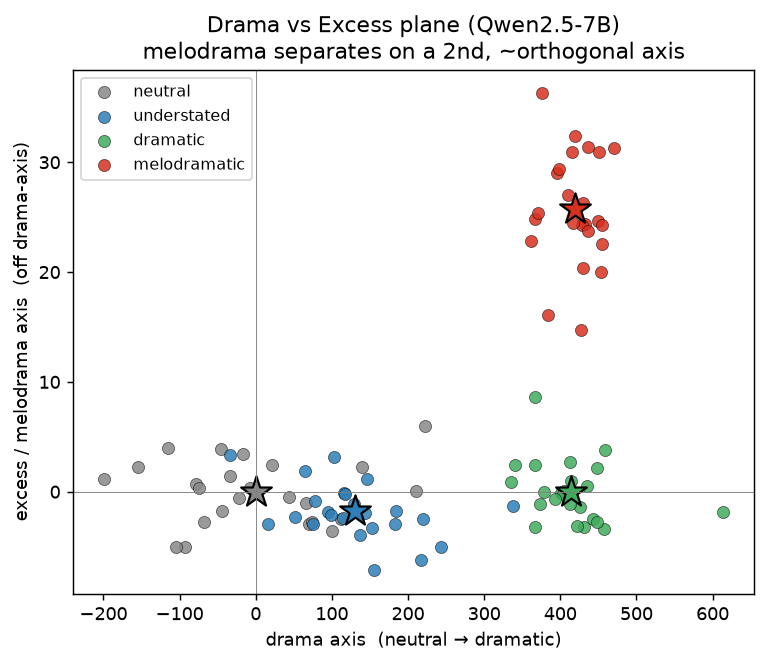
\includegraphics[width=0.55\linewidth]{figures/drama_excess_plane.png}
\caption{Dramatic (green) and melodramatic (red) items sit at the {\em same} drama-axis value but separate on a second, near-orthogonal excess axis (\qwenbig, final layer). Melodrama is off-axis, not further along it.}
\label{fig:excess}\end{figure}

\para{E2: the drama subspace is low-rank but multi-dimensional.} If drama were a single axis, the eight drama subconcepts (suspense, pathos/grief, spectacle, stakes, sincerity, excess/sentimentality, shock, restraint) would collapse onto one direction (participation ratio $\mathrm{PR}=1$); if they were unrelated, they would fill the space ($\mathrm{PR}\approx 8$). We find neither. The PR of the eight subconcept directions rises with depth to $\sim\!5.6$ in \qwenbig\ and $\sim\!5.9$ in \qwensmall\ (\tabref{tab:e1}, last column; \figref{fig:geometry}(b))---far below the random ceiling of $\sim\!8$ but well above $1$. Drama is a genuine {\em low-dimensional space} of features, not a single axis. The subconcept cosine structure is interpretable (\figref{fig:geometry}(c)): shock and suspense correlate, while pathos/grief and restraint anti-correlate, matching the intuition that built-up tension and emotional excess pull in opposite directions from quiet understatement.

\begin{figure}[t]\centering
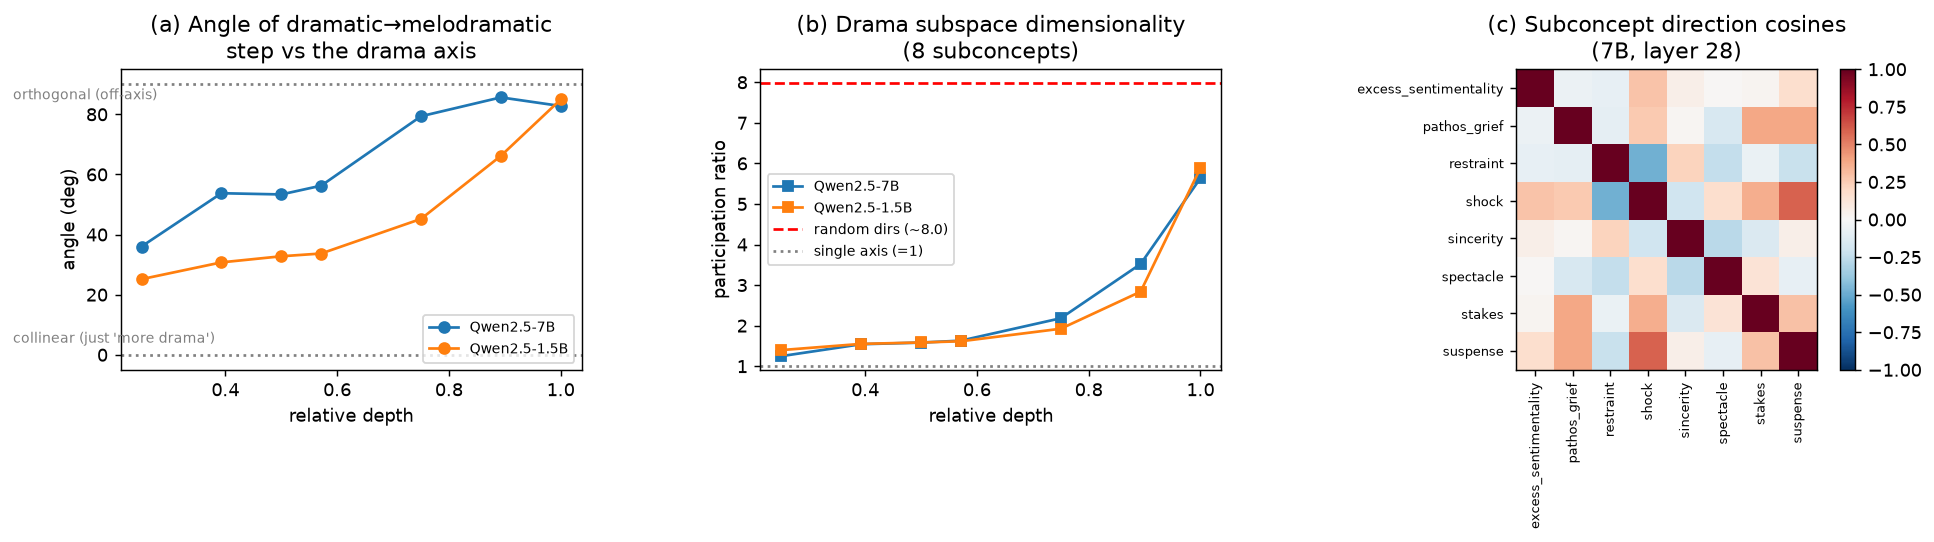
\includegraphics[width=\linewidth]{figures/e1_e2_geometry.png}
\caption{(a) The dramatic$\to$melodramatic step rotates from near-collinear to $\sim$80--86$^\circ$ with depth in both \qwenbig\ and \qwensmall; (b) the 8-subconcept participation ratio rises to $\sim$5.6--5.9, far below the random ceiling ($\sim$8) but well above a single axis (1); (c) interpretable subconcept cosine structure (shock$\leftrightarrow$suspense correlate; pathos/grief$\leftrightarrow$restraint anti-correlate).}
\label{fig:geometry}\end{figure}

\para{E3: reader variation is a threshold, not a direction.} Having shown the construct is multi-dimensional, we ask whether {\em readers} exploit those extra dimensions---whether disagreement is a reader-specific {\em direction} in the drama subspace (H2) or merely a per-reader {\em threshold} on a shared axis (H1). We fit a nested ladder of logistic models predicting each rater's binary drama label from text activations, evaluating on text-disjoint held-out items across $70$ \goemotions\ readers. \Mzero\ is a single shared axis; \Mone\ adds a per-reader threshold (intercept); \Mtwo\ adds a per-reader gain (slope); \Mthree\ lets each reader choose their own weight vector inside the drama subspace.

The transferred-corpus subspace (\dramacorpus, layer 21; \tabref{tab:e3transfer}, \figref{fig:e3}) tells the story cleanly. The decisive lift comes from the per-reader {\em threshold}: \Mzero\ at $0.510$ jumps to $0.619$ at \Mone. Everything after is flat---per-reader gain reaches only $0.622$ and a full reader-specific direction in the 9-D subspace reaches $0.623$. The added direction buys $\Delta(\Mthree-\Mtwo)=+0.0006$, exactly matching the shuffled-reader null of $+0.0006$ ($z=-0.5$): the gain is pure model capacity, present even when reader identities are randomized. The reader-weight matrix is low-rank ($\mathrm{PR}=3.25$ of $9$; \figref{fig:e3}, right), \ie\ what little reader-to-reader weight variation exists lives in a few shared dimensions, not in idiosyncratic per-reader directions.

\begin{table}[t]\centering
\caption{E3 nested held-out AUROC on a transferred \dramacorpus\ subspace (\qwenbig, layer 21, 70 readers, text-disjoint). The decisive lift is the per-reader threshold (\Mone); adding a reader-specific direction (\Mthree) matches the shuffled-reader null. Best simple model in \textbf{bold}.}
\label{tab:e3transfer}
\begin{tabular}{@{}lcc@{}}\toprule
Model & What it adds & Held-out AUROC \\\midrule
\Mzero shared single axis & --- & 0.510 \\
\Mone + per-reader threshold & reader intercept & \textbf{0.619} \\
\Mtwo + per-reader gain & reader slope (1-axis) & 0.622 \\
\Mthree + per-reader direction & weight vector in 9-D subspace & 0.623 \\
\bottomrule\end{tabular}\end{table}

The in-domain PCA subspace ($K{=}30$; \tabref{tab:e3indomain}, \figref{fig:e3b}) is the fairer test, since the drama directions are estimated from the same activation distribution the readers are evaluated on, and it reproduces the pattern at higher absolute AUROC. At layer 21, \Mzero\ scores $0.660$ and the per-reader threshold (\Mone) drives the jump to $0.700$; the shared $K$-dim subspace (\MtwoK) barely helps beyond one axis at $0.701$, and the reader-specific direction (\Mthree) reaches only $0.708$. The reader-direction effect $\Delta(\Mthree-\MtwoK)=+0.0076$ is {\em identical} to the shuffled-reader null of $+0.0076$ ($z=1.0$). Layer 28 repeats this ($0.641\to0.686\to0.687\to0.691$; $\Delta=+0.0046$ real vs.\ $+0.0046$ null, $z=-0.2$). Across both layers the decisive lift is $\Mzero\to\Mone$ ($+0.04$ to $+0.11$), the shared full subspace adds $\sim\!+0.001$ beyond one axis, and the reader-specific direction adds nothing beyond the null. \figref{fig:e3b}(b) shows the real reader-direction effect lying directly on top of the shuffled-reader null distribution. The cross-model replication in \qwensmall\ (layer 21) is identical in shape: $0.661\to0.702\to0.703\to0.711$, with $\Delta(\Mthree-\MtwoK)=+0.0084$ matching the null of $+0.0084$ ($z=0.28$). Reader disagreement is a threshold on a shared axis, not a reader-specific direction.

\begin{table}[t]\centering
\caption{E3 nested held-out AUROC on the in-domain PCA drama subspace ($K{=}30$), \qwenbig. The per-reader threshold (\Mone) drives the gain; the shared $K$-dim subspace barely helps beyond one axis, and the reader-specific direction (\Mthree) adds only the shuffled-reader null. Decisive threshold row in \textbf{bold}.}
\label{tab:e3indomain}
\begin{tabular}{@{}lcc@{}}\toprule
Model & Layer 21 & Layer 28 \\\midrule
\Mzero shared 1 axis & 0.660 & 0.641 \\
\Mone + reader threshold & \textbf{0.700} & \textbf{0.686} \\
\MtwoK shared $K$-dim + threshold & 0.701 & 0.687 \\
\Mthree reader-specific $K$-dim direction & 0.708 & 0.691 \\
$\Delta(\Mthree-\MtwoK)$ real vs.\ null & $+0.0076$ vs.\ $+0.0076$ ($z{=}1.0$) & $+0.0046$ vs.\ $+0.0046$ ($z{=}{-}0.2$) \\
\bottomrule\end{tabular}\end{table}

\begin{figure}[t]\centering
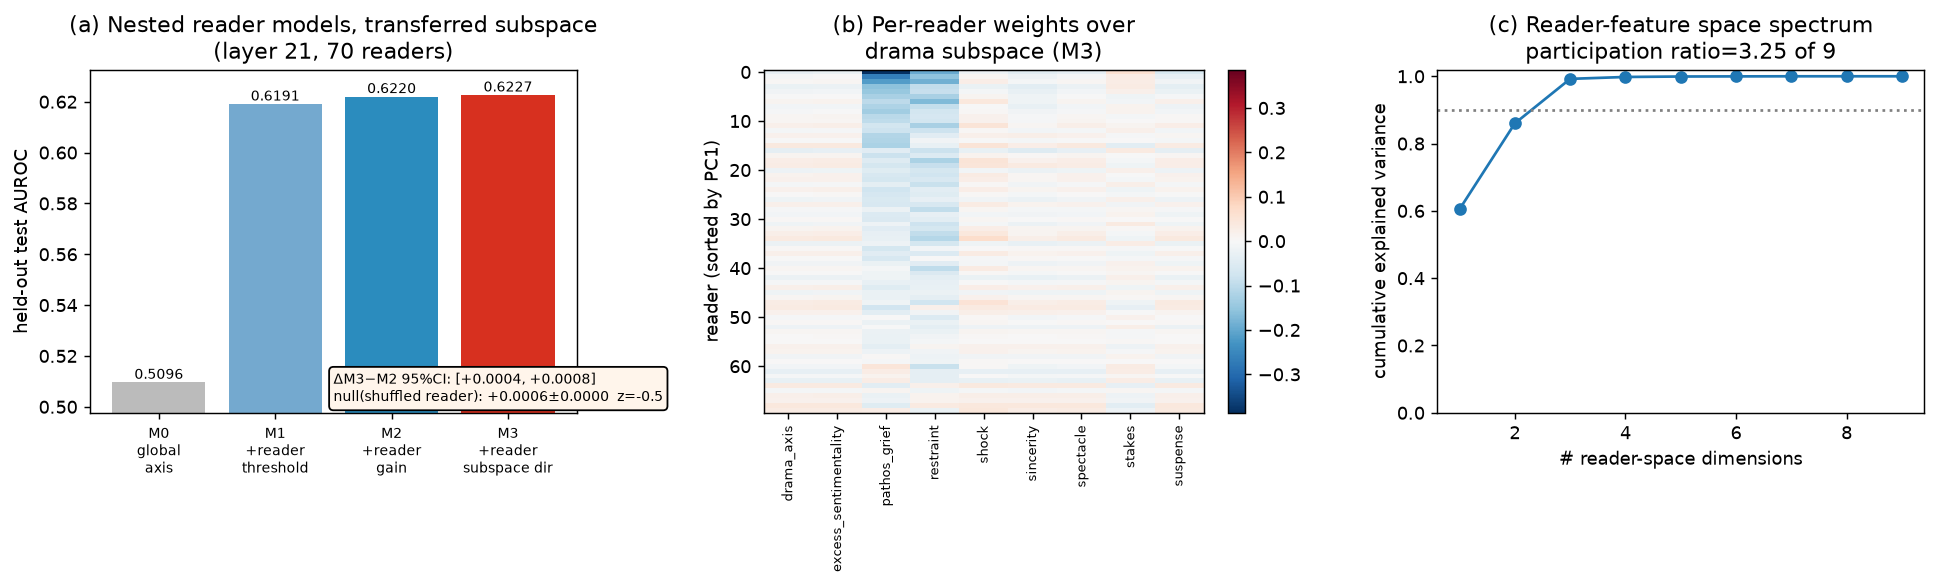
\includegraphics[width=\linewidth]{figures/e3_reader_models.png}
\caption{Transferred-subspace nested ladder (left), per-reader weights over the drama subspace (center), and the reader-feature spectrum (right, $\mathrm{PR}=3.25$ of 9). The per-reader threshold (\Mone) captures nearly all the gain; \Mthree\ adds only the null.}
\label{fig:e3}\end{figure}

\begin{figure}[t]\centering
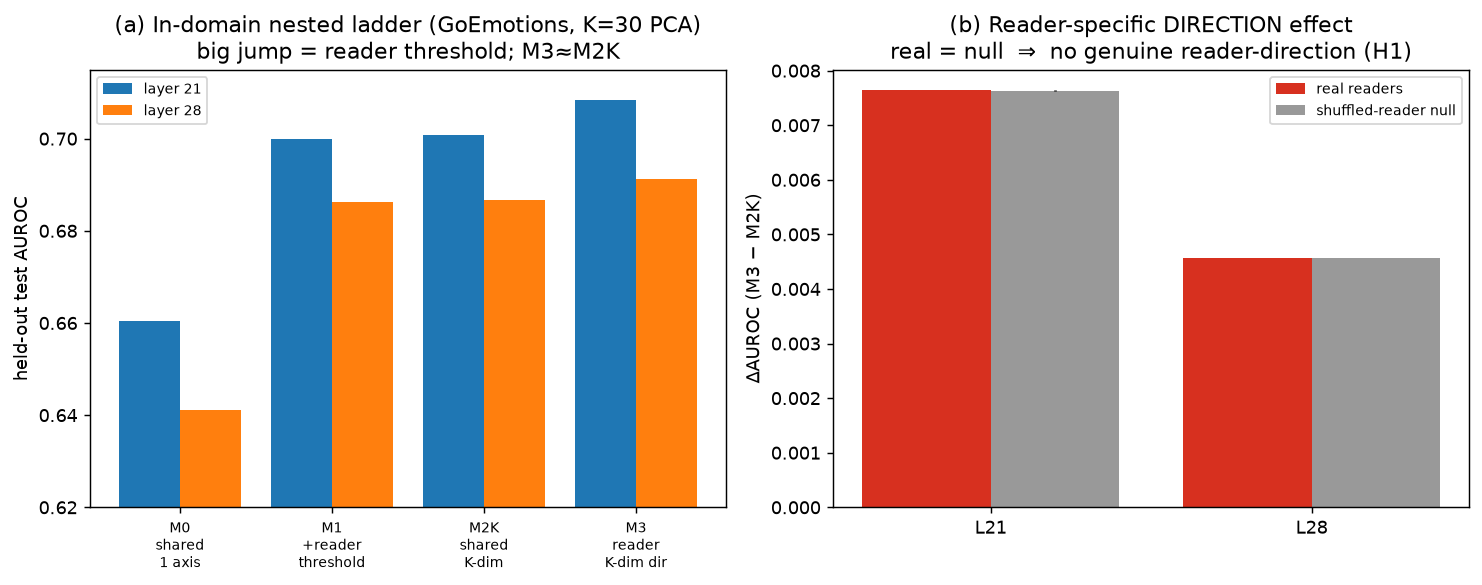
\includegraphics[width=\linewidth]{figures/e3b_indomain.png}
\caption{(a) In-domain nested ladder at layers 21/28---the big jump is the per-reader threshold (\Mzero$\to$\Mone) and \Mthree$\approx$\MtwoK; (b) the reader-specific direction effect $\Delta(\Mthree-\MtwoK)$ equals the shuffled-reader null, so it is pure model capacity, not genuine reader-direction structure.}
\label{fig:e3b}\end{figure}

\para{E4: prompting a persona does not rotate the drama axis.} Finally we re-derive the drama axis under six prompted reader personas (cynic, romantic, stoic, thrill-seeker, critic, neutral) using the chat template and a system persona. If different readers read along different directions, persona-conditioned axes should diverge. They do not: pairwise cosine between persona drama axes is $\geq 0.974$ (mean $0.99$), \ie\ all six personas recover essentially the same direction (\figref{fig:persona}(a)). The register ordering (neutral $<$ understated $<$ dramatic $<$ melodramatic) is unchanged across all personas (\figref{fig:persona}(b)). Prompting a reader shifts where the projection falls and where the threshold sits, but it does not rotate the axis---consistent with the E3 verdict that reader variation is a shared-axis threshold.

\begin{figure}[t]\centering
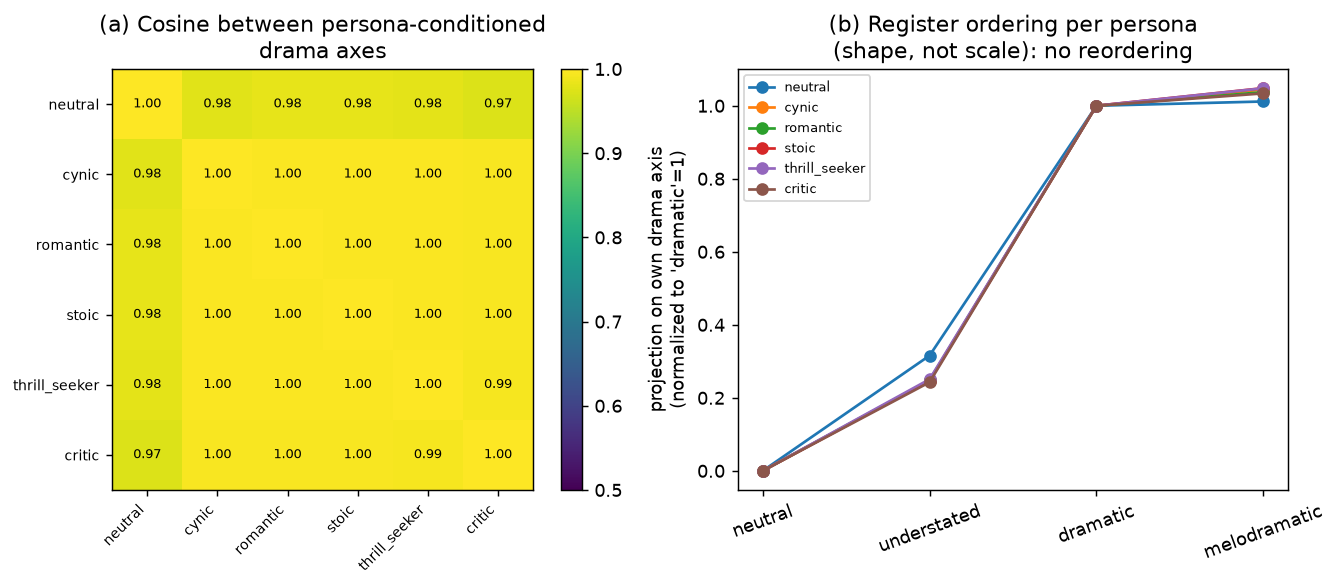
\includegraphics[width=\linewidth]{figures/e4_persona.png}
\caption{(a) Pairwise cosine between persona-conditioned drama axes is $\geq 0.974$ (mean $0.99$); (b) the register ordering is unchanged across personas. Prompting a reader shifts the projection/threshold, not the axis.}
\label{fig:persona}\end{figure}

Taken together, the construct is multi-dimensional---drama and melodrama occupy distinct, near-orthogonal directions (E1) within a low-rank but multi-dimensional subspace (E2)---yet readers share that geometry and differ almost entirely in {\em where} they place the threshold, not in {\em which} direction they read (E3, E4).

\section{Discussion}\label{sec:discussion}

\para{A clean dissociation.} Our experiments separate two questions that the phrase ``different kinds of drama'' quietly conflates. First, is the drama \emph{construct} one thing or many? We find it is genuinely multi-dimensional and \emph{shared} across readers: drama decodes perfectly (AUROC $1.000$, \tabref{tab:e1}), yet melodrama is not just more drama---the dramatic$\to$melodramatic step rotates to $83^\circ$ from the drama axis at the final layer (\tabref{tab:e1}), and an eight-subconcept subspace reaches participation ratio $\sim$$5.6$ (vs.\ $\sim$$8.0$ random, vs.\ $1$ for a single axis; \figref{fig:geometry}). Second, do different \emph{people} read along different directions, or do they slide a threshold along the same axis? Here the answer is overwhelmingly the threshold: a per-reader intercept lifts held-out AUROC from $0.660$ to $0.700$ (in-domain, layer 21; \tabref{tab:e3indomain}), while letting each reader choose her own direction in a $30$-dimensional drama subspace adds only $+0.0076$---exactly the shuffled-reader null ($z\!=\!1.0$, n.s.). So ``different kinds of drama'' are \emph{content directions} (earned drama vs.\ melodramatic excess), but ``different people''---for both \goemotions{} intensity disagreement and six prompted personas---are a \emph{sliding threshold} on a fixed, shared axis.

\para{Why this is not trivial.} A reader who suspects drama is multi-dimensional and reader-dependent could be right two ways, and only one survives. The construct could carry an off-axis excess dimension, which it does: \Secref{sec:results} (E1/E2) confirms melodrama as a near-orthogonal excess direction. Or---the stronger H2 claim---individual readers could decode drama from \emph{personal} directions inside that subspace. They do not. The reader-direction model fails its pre-registered control: its gain matches the shuffled-reader permutation null at every layer and scale (layer 21 $+0.0076$ vs.\ $+0.0076$; layer 28 $+0.0046$ vs.\ $+0.0046$; $1.5$B $+0.0084$ vs.\ $+0.0084$), meaning the apparent improvement is pure model capacity that persists even when reader identities are randomized. The multidimensionality lives in the \emph{stimulus} representation and is available to every reader equally; what individuals select is a threshold, not a private axis. Six personas confirm this from the prompt side: their re-derived drama axes are essentially identical (pairwise cosine mean $0.99$, min $\geq0.974$; \figref{fig:persona}), shifting projection and threshold but never the direction.

\para{Relation to prior work.} The shared-axis half of our result sits comfortably with low-dimensional steerable affect manifolds \citep{reichman2025emotions} and with sentiment as essentially one linear direction \citep{tigges2023linear}: a single drama axis decodes near-perfectly and is stable across personas. The reader half refines \citet{orlikowski2025beyond}: reader effects are real and learnable---our $M_0\!\to\!M_1$ threshold lift of $+0.04$ to $+0.11$ is the dominant gain---but they are not captured by low-dimensional demographic structure, and we add that they are not a reader-specific \emph{representational} direction either. The melodrama-as-excess axis is a drama-specific instance of concept-cone and subspace geometry \citep{wollschlager2025geometry}: even an affective construct that decodes as ``one thing'' needs more than one dimension to separate its kinds---just not a reader-conditioned one.

\para{Limitations.} Our verdict is bounded by its operationalizations. For \goemotions{} we operationalize drama as perceived arousal/intensity, and reader labels are binary high-arousal indicators; the H1 conclusion is therefore ``no \emph{detectable} reader-specific direction,'' not proof of absence---graded or continuous scales could expose direction effects the binary cannot resolve. The controlled \dramacorpus{} consists of LLM-authored register variants, and the stimuli are Claude-authored; both were adversarially blind-validated ($290/290$ at $100\%$ agreement), and crucially the subjects of study---Qwen activations and human raters---are independent of the generator, but generator priors could still shape the excess axis. We study one model family (Qwen2.5), replicated across $1.5$B and $7$B and across layers, but cross-family generalization (Llama, Gemma) is untested. Finally, activations are mean-pooled over tokens; token-level probes, SAE decompositions, and causal steering are planned but not run here.

\para{Broader implications.} The practical upshot is that personalizing affect judgments to a reader is often cheap. If individual variation in what counts as ``dramatic'' is mostly a threshold shift on a shared axis rather than steering within a multi-dimensional subspace, then adapting to a reader can be a one-parameter calibration rather than learning a per-user representation---a far smaller and more auditable intervention. At the same time, the construct's own multidimensionality is consequential: earned drama and melodramatic excess occupy nearly orthogonal directions, so moderation, recommendation, and criticism systems that collapse them into a single ``intensity'' score will systematically conflate genuine stakes with sentimentality. The lesson cuts both ways---model the \emph{content} as multi-dimensional, but the \emph{reader} as a movable threshold.

\section{Conclusion}\label{sec:conclusion}

We asked how an LLM represents what different people find dramatic, and we find a split answer that cleanly separates the structure of the construct from the structure of disagreement. On the construct side, the model represents drama as a low-dimensional \emph{space} of features rather than a single axis: drama itself decodes perfectly (AUROC $1.000$), but melodrama is not just more drama---the dramatic$\to$melodramatic step rotates to $\sim$83 degrees from the drama axis in the deepest layers (\Tabref{tab:e1}), dramatic and melodramatic texts sit at the same drama-axis value while splitting along an orthogonal \emph{excess} direction (\figref{fig:excess}), and an 8-subconcept subspace has participation ratio rising to $\sim$5.6 ($\sim$5.9 in \qwensmall), far above a single axis (\figref{fig:geometry}). ``Different kinds of drama'' are therefore genuine and geometric. On the disagreement side, the picture is the opposite: per-reader variation is overwhelmingly a \emph{threshold} on a shared drama axis. Adding a per-reader threshold lifts held-out AUROC from $0.510$ to $0.619$ (transferred subspace) and from $0.660$ to $0.700$ (in-domain), while a shared full subspace barely helps beyond one axis ($\sim+0.001$) and letting each reader pick their own \emph{direction} adds exactly the shuffled-reader null ($\Delta$AUROC $+0.0076$ real vs.\ $+0.0076$ null, $z\!\approx\!1.0$, n.s.; \Tabref{tab:e3indomain}, \figref{fig:e3b}). Six prompted personas leave the drama axis essentially fixed (pairwise cosine $\geq 0.974$, mean $0.99$; \figref{fig:persona}). The strong multi-dimensional reader hypothesis is not supported, for either natural disagreement or prompted personas. {\bf The key takeaway: drama's multidimensionality lives in the shared content, while inter-reader differences are mostly about where the threshold sits.}

Several directions would give the reader-direction hypothesis its strongest possible chance and pin down the excess axis causally. First, our \goemotions\ labels are binary high-arousal indicators, so our verdict is ``no \emph{detectable} reader-specific direction''; a purpose-built, graded, multi-reader \emph{drama} rating set could expose reader-specific structure that a binary indicator cannot resolve. Second, causal steering along the drama and excess axes \citep{wollschlager2025geometry} would confirm that the two directions are independent under intervention, not merely in observed geometry, and SAE or feature-circuit localization \citep{marks2024sfc} could identify the components that implement the excess direction. Third, our results hold across \qwensmall\ and \qwenbig\ and across layers and subspace dimensions, but cross-family replication on Llama and Gemma is needed to rule out a Qwen-specific geometry. Finally, prompted personas did not rotate the drama axis; a natural next test is whether \emph{fine-tuned} reader embeddings---rather than system prompts---can rotate the axis where personas could not, which would be the most direct route from a shared-threshold account back toward genuinely reader-specific directions.


\bibliography{references}

\end{document}
